% !TEX encoding = Windows Cyrillic
\documentclass[a4paper, 11pt]{article}
\usepackage[tikz]{newlistok}

\УвеличитьШирину{1.5truecm}
\УвеличитьВысоту{2.5truecm}

\begin{document}

\Заголовок{Приближение действительных чисел рациональными II:
Уравнение Пелля}
\НомерЛистка{NT-2}
\ДатаЛистка{2022.01}
%\Оценки{99/99/99}
\СоздатьЗаголовок

\def\mtrx#1#2#3#4{\begin{pmatrix}#1 & #2 \\ #3 & #4\end{pmatrix}}
\def\vctr#1#2{(#1\;#2)}

% limited rel (Арсен) 07.09 (?); www-rel: 29.12.2013
% минимум третья попытка собрать листок примерно про одно и то же
% опирается на листок про цепные дроби
\опр
Пусть $d$~--- целое число, свободное от квадратов. \emph{Нормой} элемента $z=x+y\sqrt d\in\Z[\sqrt d]$ называется целое число $N(z)=x^2-dy^2$.
\копр




\задача
Норма мультипликативна: $N(zw)=N(z)N(w)$.
\кзадача






\опр
Пусть $d$~--- целое число, свободное от квадратов. Диофантово уравнение $x^2-dy^2=1$ называется \emph{уравнением Пелля}.

Решением уравнения Пелля мы будем называть как пару целых чисел $\vctr xy$, так и~соответствующий элемент единичной нормы $x+y\sqrt d$ кольца $\Z[\sqrt d]$.
\копр




\задача
\пункт Если уравнение Пелля имеет нетривиальное (отличное от $\vctr{\pm1}0$) решение, то оно имеет бесконечно много решений.

\пункт Если уравнение Пелля имеет нетривиальное решение, то группа его положительных решений изоморфна $\Z$.
\кзадача





\УстановитьГраницы{0mm}{45mm}
\сзадача
\righttikz{0mm}{0mm}{
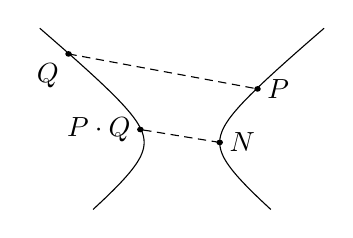
\begin{tikzpicture}[yscale=.4,xscale=.48]
%    \begin{axis}[axis x line=none, axis y line=none, no markers]
 %       \addplot {sqrt(1+x^2)};
 %       \addplot {-sqrt(1+x^2)};
 %   \end{axis}
\draw[scale=1,domain=-1.5:2,smooth,variable=\t] plot ({ cosh(\t)},{sinh(\t)});
\draw[scale=1,domain=-1.5:2,smooth,variable=\t] plot ({-cosh(\t)},{sinh(\t)});
\filldraw[black] (1,0) circle (2pt) node[right] {$N$};
\filldraw[black] (2,1.7) circle (2pt) node[right] {$P$};
\filldraw[black] (-3,2.81) circle (2pt) node[below left] {$Q$};
\draw[densely dashed] (-3,2.81)--(2,1.7);
\draw[densely dashed] (1,0)--(-1.1,0.41);
\filldraw[black] (-1.1,0.41) circle (2pt) node[left] {$P\cdot Q$};
\end{tikzpicture}}
Пусть $N=\vctr10$; $P$ и~$Q$~--- пара точек на гиперболе $x^2-dy^2=1$. Проведем через точку $N$ секущую, параллельную хорде $PQ$.
\\\пункт Эта секущая пересекает гиперболу еще ровно в~одной точке\footnote{Если отрезок $PQ$ оказался вертикальным, то надо считать, что вторая точка совпадает с~$N$ (в~этом случае наша ``секущая'' как раз касается гиперболы).}.
\\\пункт Построенная точка соответствует произведению элементов единичной нормы, соответствующих точкам $P$ и~$Q$.
\кзадача
\ВосстановитьГраницы





\задача
Решите уравнение \пункт $x^2-3y^2=-2$;\quad \пункт $x^2-3y^2=-1$.
\кзадача






\задача
Найдите формулу для $k$-го треугольного числа, являющегося точным квадратом.
% $\bigl(\frac{(3+2\sqrt2)^k-(3-2\sqrt2)^k}{4\sqrt2}\bigr)^2
\кзадача






\опр
Значением \emph{квадратичной формы} с~(симметричной) матрицей $Q$ на векторе~$v$ называется число $(v,Qv)$.
Таким образом, матрица $\mtrx a{b/2}{b/2}c$ задает квадратичную форму $ax^2+bxy+cy^2$.
\копр




\сзадача
Отображение $Q$ квадратично тогда и~только тогда, когда отображение $(u,v)\mapsto Q(u+v)-Q(u)-Q(v)$ билинейно\footnote{Это можно считать определением квадратичного отображения~--- а~доказывать, соответственно, что любое квадратичное отображение задается некоторой симметричной матрицей.}.
\кзадача






\задача
Как меняется квадратичная форма при замене координат с~матрицей~$C$?
\кзадача






\задача
\пункт Существует лишь конечное число целочисленных квадратичных форм с~$ac<0$ и~фиксированным дискриминантом $-d<0$.

\пункт Целочисленная квадратичная форма $\mtrx 100{-d}$ имеет нетривиальный автоморфизм (т.\,е. существует обратимая целочисленная замена координат, при которой эта форма не меняется). % отличная от $\mtrx{-1}001$.

{\small Указание. Рассмотрите алгоритм вытягивания носов для $\sqrt d$.\par}

\пункт Уравнение Пелля имеет нетривиальное решение.

\пункт Разложение числа $\sqrt d$ в~цепную дробь периодично.

\спункт Разложение иррационального числа в~цепную дробь периодично тогда и~только тогда, когда это квадратичная иррациональность (``теорема Лагранжа'').
\кзадача






\задача
У~числа $\sqrt d$  бесконечно много приближений, таких что $|\alpha-\frac pq|<\smash{\frac1{(2\sqrt d-\varepsilon)q^2}}$.
\кзадача






\сзадача
\пункт Период цепной дроби числа $\sqrt d$ без последнего числа~--- палиндром.

\пункт Уравнение $x^2-dy^2=-1$ имеет решение тогда и~только тогда, когда период цепной дроби числа $\sqrt d$ имеет нечетную длину.
\кзадача











 \ЛичныйКондуит{0mm}{6.5mm}
% \GenXMLW
\end{document} 